\chapter{\\METHODOLOGY}

This chapter describes in rigorous detail how the research was conceptualized, designed, and executed to address the core problem statement. It covers the overarching research design philosophy, the meticulous requirements analysis process involving target users, the specific user-centred design (UCD) methodology applied to the interface, the agile software development approach utilized for the full-stack engineering, and the strict empirical evaluation protocol deployed to measure success.

% ─────────────────────────────────────────────────────────────────────────────
\section{Overview}

\textbf{Research Design Paradigm.}

This research fundamentally adopts a \emph{design science} paradigm~\cite{sommerville2016}, a highly pragmatic methodological approach well-suited for software engineering and information systems research. In design science, the primary contribution to knowledge is not merely a theoretical observation, but rather the creation, thorough description, and rigorous evaluation of an innovative artefact—in this case, the comprehensive, AI-assisted H5P interactive video platform. Design science research is specifically appropriate for projects that aim to solve a concrete, identified problem for a defined stakeholder group (university instructors at VNU-HCM) by building and evaluating a purposeful software artefact. The methodology mandates that the artefact must be novel, must solve the problem effectively, and its utility must be rigorously demonstrated through empirical evaluation.

The research architecture seamlessly combines two distinct, chronological methodological phases:

\begin{enumerate}
  \item \textbf{Constructive phase (Engineering \& Design).} During this phase, extensive user requirements are elicited from the target demographic. The system architecture is designed from the ground up to support high-performance web delivery. The frontend user interface and backend REST APIs are implemented, and crucially, the highly complex, multi-stage AI pipeline (encompassing transcript extraction, prompt formatting, LLM inference, and strict Zod validation) is engineered and integrated into the H5P ecosystem.
  
  \item \textbf{Evaluative phase (Empirical Measurement).} Once the platform reaches a stable, feature-complete release candidate state, a highly controlled comparative usability study is conducted. This study empirically measures the new artefact's performance directly against the incumbent, widely used WordPress-based H5P workflow. The evaluation relies on four primary quantitative metrics: objective task completion rate, precise time-on-task, observed error frequency, and the standardized System Usability Scale (SUS) score, supplemented by rich qualitative feedback.
\end{enumerate}

\textbf{Software Development Methodology.}

An \emph{agile software development methodology} was explicitly chosen and rigorously applied throughout the constructive phase, utilizing short, focused iterative cycles (sprints) of two to three weeks each~\cite{beck2001}. Each sprint was required to produce a stable, testable increment of the platform. Continuous integration and informal cognitive walkthroughs at the end of each cycle provided immediate feedback that directly informed the subsequent design iteration. This flexible approach was specifically chosen because the complex technical interaction between the generative AI pipeline, the strict schema requirements of the H5P libraries, and the fluid nature of human-computer interaction in the authoring workflow could not be fully, rigidly specified in advance. Crucial usability requirements and edge-case technical constraints emerged organically only during active implementation and required immediate architectural pivots.

% ─────────────────────────────────────────────────────────────────────────────
\section{User requirement analysis}
\label{sec:requirements}

\textbf{User Research and Elicitation.}

The foundational step of the constructive phase involved deep qualitative user research to accurately capture the specific pain points of the target demographic. Semi-structured, informal interviews were conducted with five diverse instructors at HCMIU, representing both technical and non-technical disciplines. These sessions revealed four highly consistent, dominant themes: 
(1) The current WordPress/H5P workflow is universally perceived as overwhelmingly complex and totally disconnected from pedagogical goals; 
(2) Authors experience severe anxiety regarding losing their work due to accidental browser reloads or plugin timeouts mid-edit; 
(3) The manual content creation process (finding timestamps, typing questions, formatting distractors) is prohibitively time-consuming; 
(4) There is massive, explicit demand for intelligent, AI-assisted scaffolding to suggest questions based on lecture content. 

A subsequent short, direct observational session was conducted where a user attempted to create a simple three-question interactive video using the baseline WordPress tool. This observation empirically confirmed the 45-to-60-minute average completion time and vividly demonstrated that constant contextual switching (losing track of the video playback position while filling out dense configuration forms) and cryptic plugin error screens were the absolute most common causes of extreme frustration and task abandonment.


\begin{figure}[H]
  \centering
  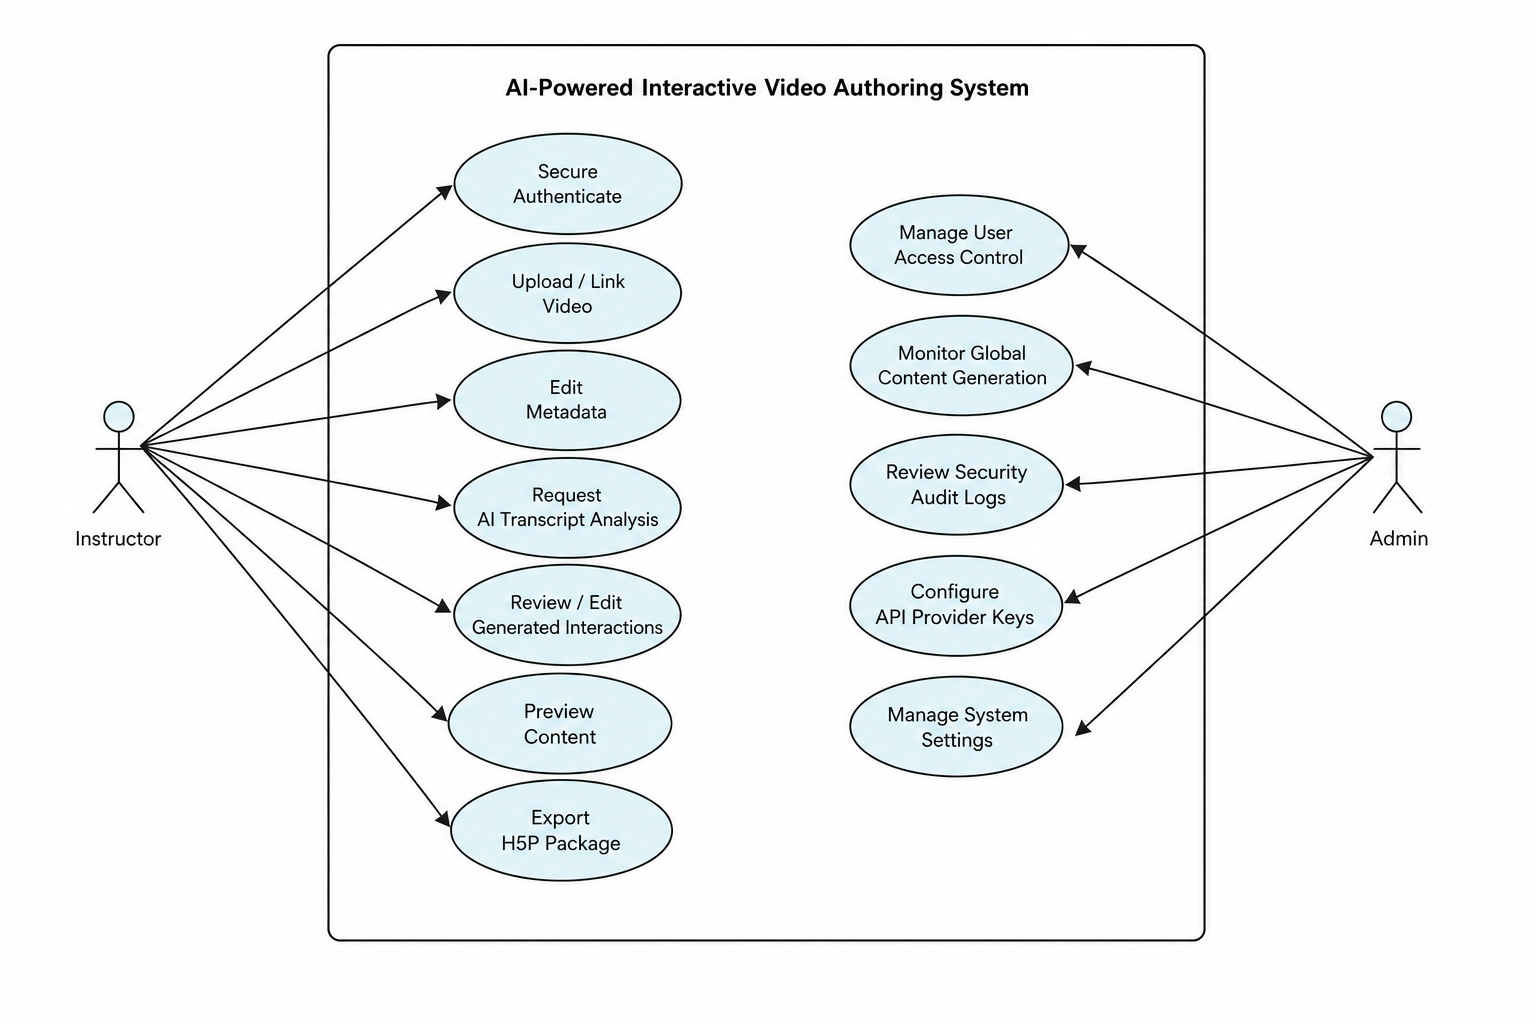
\includegraphics[scale=0.3]{thesis 3/images/Usecase.png}
  \caption{Use case diagram}
  \label{fig:usecase}
\end{figure}

\subsection{Functional and Non-Functional Requirements}

The qualitative research was subsequently translated into a strict specification of functional requirements to guide the engineering effort:
\begin{itemize}
  \item \textbf{Authentication \& Access:} Secure user account creation, JWT-based stateless sessions, strict role-based access control (RBAC), and email verification workflows.
  \item \textbf{Media Management:} Robust video file upload handling (up to 500MB) and seamless YouTube URL import, coupled with a highly responsive, timeline-based H5P visual editor and instant real-time content preview.
  \item \textbf{H5P Core Functionality:} Full manual and AI-assisted support for six pedagogical H5P interaction types, with a guaranteed one-click \texttt{.h5p} package export mechanism.
  \item \textbf{AI Pipeline Integration:} Advanced transcript extraction (Whisper/VTT/YouTube) feeding an AI analysis pipeline that produces strictly validated H5P JSON suggestions, complete with Server-Sent Events (SSE) for real-time progress streaming to the UI.
  \item \textbf{Authoring Workflow:} A streamlined accept/reject/edit workflow interface for reviewing AI suggestions before server-side injection into the permanent H5P content database.
  \item \textbf{Administration:} Comprehensive admin dashboards for user management, system health monitoring, and a stubbed architecture for optional LTI 1.3 LMS deep-linking integration.
\end{itemize}

\textbf{Non-Functional Requirements.}

Non-functional requirements rigorously govern the critical quality attributes, performance baselines, and security constraints of the engineered system. These are strictly detailed in Table~\ref{tab:nonfunc_reqs}.

\begin{table}[H]
  \centering
  \begin{tabularx}{\linewidth}{l >{\raggedright\arraybackslash}p{2.2cm} X}
    \toprule
    \textbf{ID} & \textbf{Category} & \textbf{Requirement Definition} \\
    \midrule
    NFR-01 & Performance & All standard REST API responses must complete within 500\,ms under a load of 50 concurrent active users. \\
    \addlinespace
    NFR-02 & Performance & Initial video upload processing (thumbnail/metadata) must complete within 30\,s for files $\leq 100$\,MB. \\
    \addlinespace
    NFR-03 & Security    & All user passwords must be securely hashed using bcrypt with a computational cost factor of at least 12. \\
    \addlinespace
    NFR-04 & Security    & Authentication tokens must utilize stateless JWT, signed with HS256, strictly expiring after 7 days. \\
    \addlinespace
    NFR-05 & Security    & All HTTP responses must enforce strict Helmet-generated security headers (CORS, CSP, XSS protection). \\
    \addlinespace
    NFR-06 & Security    & All API endpoints must aggressively validate and type-check input payloads using Zod schemas. \\
    \addlinespace
    NFR-07 & Reliability & The AI system must handle failure of Claude/Ollama gracefully, returning errors rather than crashing the process. \\
    \addlinespace
    NFR-08 & Usability   & The final platform iteration must achieve a minimum System Usability Scale (SUS) score of 70. \\
    \addlinespace
    NFR-09 & Usability   & The first-time task completion rate for creating an interactive video must definitively exceed 80\%. \\
    \addlinespace
    NFR-10 & Compatibility & Exported \texttt{.h5p} packages must be 100\% valid for Moodle 4.x and Canvas LMS environments. \\
    \bottomrule
  \end{tabularx}  
  \small
  \caption{Critical Non-functional requirements driving system architecture}
  \label{tab:nonfunc_reqs}
\end{table}

% ─────────────────────────────────────────────────────────────────────────────
\section{System Design}
\label{sec:architecture}

\textbf{Architectural Overview and Topologies.}

The platform is engineered using a modern, highly scalable three-tier architecture that completely separates the presentation layer from the business logic and data persistence layers~\cite{bass2012}. 
The \emph{presentation tier} is a highly dynamic, Single-Page Application (SPA) built with React 18, Vite, and Zustand for complex global state management. 
The \emph{application tier} consists of a robust Express.js REST API running on a Node.js runtime, acting as the central orchestrator for all business logic, H5P library rendering, and AI pipeline routing. 
The \emph{data tier} utilizes a fast, file-based SQLite database managed via the Sequelize Object-Relational Mapper (ORM), ensuring rapid local development while remaining easily migratable to PostgreSQL for massive institutional deployments. 
External service dependencies are strictly limited to necessary APIs: Groq (serving as the primary, ultra-fast cloud AI inference engine), the Anthropic Claude API (acting as a highly capable cloud fallback), Ollama (providing critical local, privacy-preserving AI fallback), and the YouTube Data API. All core H5P processing runs entirely within the local server process, eliminating reliance on third-party H5P SaaS providers.

\begin{figure}[H]
  \centering
  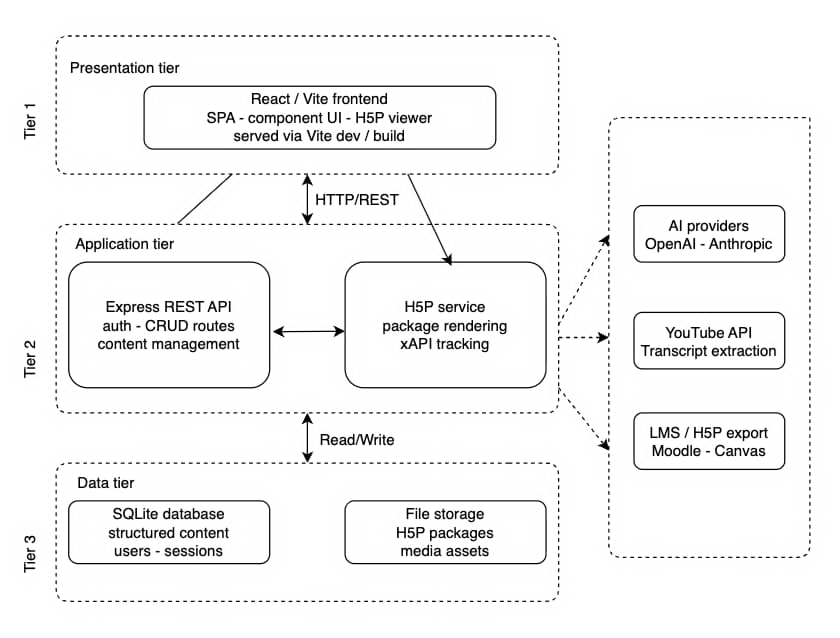
\includegraphics[scale=0.5]{thesis 3/images/Three-tỉer system.jpeg}
  \caption{Three-tier system architecture}
  \label{fig:architecture}
\end{figure}

The overarching design goals driving this architecture were: strict separation of concerns via a heavily versioned REST API; total AI-provider independence using a sophisticated, prioritized provider chain that forces uniform JSON output shapes regardless of the underlying LLM; absolute H5P library isolation using the official Lumi server package to guarantee cross-LMS compatibility; and a completely stateless backend design utilizing JWT-based session tokens to enable simple horizontal scaling behind a load balancer.

\textbf{API Route Structure and Controller Logic.}

The REST API is logically organized under the \texttt{/api/v1/} prefix, with strict middleware enforcement for authentication and rate-limiting applied at the router level. Table~\ref{tab:api_routes} exhaustively lists the primary functional route groups and their core responsibilities.

\begin{table}[H]
  \centering
  \begin{tabularx}{\linewidth}{
    >{\raggedright\arraybackslash}p{3.2cm} % Fixed width for routes
    >{\raggedright\arraybackslash}p{2cm}   % Fixed width for methods
    X                                      % Flexible space for descriptions
  }
    \toprule
    \textbf{Prefix} & \textbf{Methods} & \textbf{Responsibility} \\
    \midrule
    \texttt{/api/auth} & POST & Handles all secure registration, login, bcrypt password verification, and JWT issuance/refresh cycles. \\
    \addlinespace
    \texttt{/api/videos} & GET, POST, PUT, DELETE & Orchestrates video file chunked uploads, YouTube URL validation, thumbnail generation, and metadata CRUD. \\
    \addlinespace
    \texttt{/api/h5p} & GET, POST, DELETE & Interfaces with the Lumi library for H5P parameter CRUD, on-the-fly zip package generation, and secure iframe rendering. \\
    \addlinespace
    \texttt{/api/ai/analyze} & POST & Triggers synchronous, non-streaming transcript analysis returning a massive JSON payload. \\
    \addlinespace
    \texttt{/api/ai/analyze- stream} & POST & Triggers asynchronous transcript analysis, holding an open SSE connection to stream questions. \\
    \addlinespace
    \texttt{/api/ai/inject} & POST & Validates and securely injects user-accepted AI suggestions directly into the SQLite H5P content store. \\
    \addlinespace
    \texttt{/api/transcript} & POST & Handles complex YouTube caption extraction, VTT parsing, and segment time normalization. \\
    \addlinespace
    \texttt{/api/admin} & GET, POST, PUT & Exposes elevated endpoints for user management and system audit logs (strictly protected by Admin RBAC). \\
    \addlinespace
    \texttt{/api/lti} & GET, POST & Implements the complex OIDC handshake required for LTI 1.3 deep-linking and LMS integration. \\
    \bottomrule
  \end{tabularx}
   \small
  \caption{Comprehensive REST API route groups and functional responsibilities}
  \label{tab:api_routes}
\end{table}

% ─────────────────────────────────────────────────────────────────────────────
\section{AI Pipeline Architecture}

The sophisticated AI pipeline stands as the defining, most complex technical contribution of this software platform. It is tasked with a highly difficult transformation: converting a raw, noisy, unstructured video transcript into a strictly validated, Bloom's-taxonomy-labelled, ready-to-render list of complex H5P interaction JSON configurations. This massive transformation is accomplished through a rigorously designed five-stage pipeline. Figure~\ref{fig:ai_pipeline} illustrates the high-level sequential data flow, and Figure~\ref{fig:seq_ai} presents the detailed actor-level sequence diagram, explicitly detailing the SSE streaming path and the critical "inject-on-accept" user workflow.

\begin{figure}[H]
  \centering
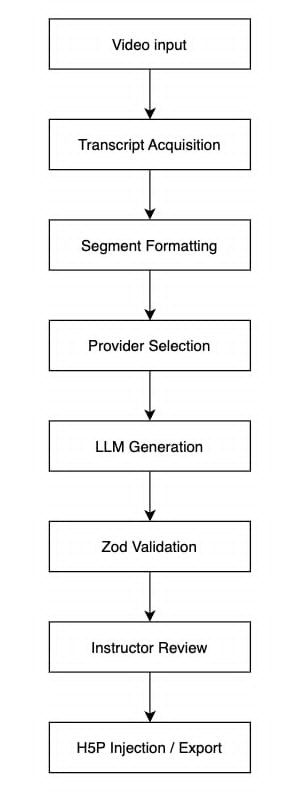
\includegraphics[scale=0.6]{thesis 3/images/AI Pipeline.jpeg}
  \caption{AI pipeline flowchart}
  \label{fig:ai_pipeline}
\end{figure}

\begin{figure}[H]
  \centering
 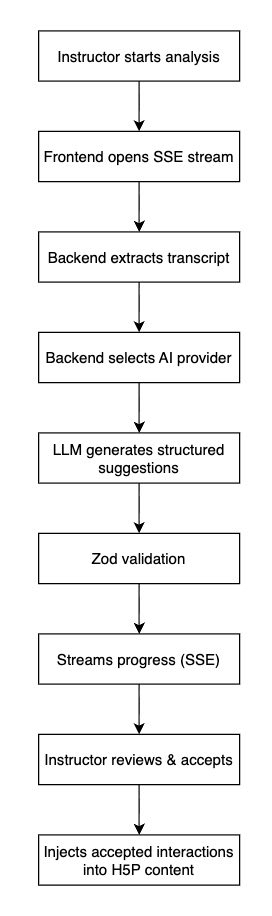
\includegraphics[scale=0.75]{thesis 3/images/AI asisted question generation.jpeg}
  \caption{AI-assisted question generation sequence diagram}
  \label{fig:seq_ai}
\end{figure}

\textbf{Stage 1: Transcript Acquisition and Normalization.}

Flawless transcript acquisition is the foundational requirement for generation accuracy. This is handled by the dedicated \texttt{transcriptExtraction.js} microservice, which robustly supports three distinct source mechanisms to ensure maximum compatibility:

\begin{enumerate}
  \item \textbf{YouTube Automatic/Manual Captions} (Primary for YouTube URLs). The system utilizes the \texttt{youtube-transcript} npm package to stealthily fetch timestamped XML caption segments directly from the internal YouTube API using the video's unique 11-character ID. These segments are instantly parsed and normalised into a strict, standard JavaScript object format: \texttt{\{start: number, end: number, text: string\}}.
  \item \textbf{Uploaded WebVTT Caption Files} (Primary for local video uploads). Instructors possess the option to manually upload a standard WebVTT (\texttt{.vtt}) or SRT file alongside their video asset. The service utilizes a robust regex-based parser to extract timing cues and text, normalizing them into the identical standard segment format.
  \item \textbf{Whisper Neural Audio Transcription} (Fallback mechanism). For uploaded video files lacking any caption data, the service automatically invokes the powerful \texttt{faster-whisper} neural network model via an asynchronous Python subprocess. It passes the absolute path of the video file and requests English/Vietnamese transcription. The resulting highly accurate JSON transcript is subsequently normalized into the standard segment format. Whisper system availability is continuously verified at server startup and reported to the frontend via the \texttt{GET /api/ai/status} health endpoint~\cite{radford2023}.
\end{enumerate}

Crucially, all three disparate sources produce the same \texttt{TranscriptSegment[]} data structure, absolutely ensuring that the downstream AI prompting stage remains entirely source-agnostic and decoupled from the extraction logic.

\textbf{Stage 2: Advanced Segment Formatting.}

The \texttt{formatSegmentsForPrompt()} utility function within \texttt{aiService.js} converts the normalized array of segment objects into a highly structured, human-readable transcript string heavily annotated with precise timestamp labels. Each individual line is formatted as follows:

\begin{lstlisting}[language={},caption={Advanced transcript segment formatting injecting raw-second timestamps}]
// Input normalized segment object: { start: 330, end: 345, text: "Photosynthesis converts light..." }
// Output formatted prompt line:
"[05:30 (330s) -> 05:45 (345s)] Photosynthesis converts light..."
\end{lstlisting}

This formatting is a critical prompt engineering decision. Each segment line deliberately embeds \emph{both} the familiar human-readable \texttt{MM:SS} format (providing the LLM with chronological context) \emph{and} the raw integer seconds enclosed in parentheses. The master system prompt explicitly and forcefully instructs the model to extract and use \emph{only} the raw seconds integer for the \texttt{startTime} and \texttt{endTime} JSON fields. This technique entirely eliminates the severe rounding errors and hallucinated timestamps that frequently occur when LLMs attempt to mathematically parse or reconstruct "MM:SS" string formats back into the integers required by the H5P player~\cite{white2023}.

\textbf{Stage 3: Two-Step AI Prompt Engineering and Question-Type Assignment}
\label{sec:stage3}
The core AI system prompt, defined as a constant in \texttt{aiService.js}, adopts an advanced two-step \emph{output automater} prompt-engineering pattern~\cite{white2023}. This pattern strategically separates high-level topic discovery from the low-level mechanical generation of question JSON. By heavily constraining the model's degrees of freedom at each distinct step, output consistency and schema adherence improve exponentially.

\subsubsection{Step 1 --- Hierarchical Topic Segmentation}In the first step, the LLM receives the heavily formatted transcript and is explicitly instructed to act as an expert instructional designer. It must produce a hierarchical topic outline rather than a flat, disconnected list of question suggestions. The strictly required output structure is a complex JSON array containing 2 to 5 top-level topics. Each topic node must carry its bounding timestamp span, a carefully assigned Bloom's taxonomy pedagogical level~\cite{anderson2001}, an estimated difficulty rating (1--3), and optionally 1 to 3 nested subtopics. Most importantly, every topic node and every subtopic node must be associated with \emph{exactly one} generated H5P question object:

\begin{lstlisting}[language={},caption={Strictly required JSON output structure for Step 1 (hierarchical topic segmentation)}]
    "topic": "Photosynthesis Overview",
    "startTime": 330,
    "endTime": 345,
    "bloomsLevel": "Remember",
    "difficulty": 1,
    "subtopics": [
      {
        "subtopic": "Light-dependent reactions",
        "startTime": 360,
        "endTime": 380,
        "bloomsLevel": "Understand",
        "difficulty": 2,
        "question": { /* Schema-compliant H5P question object */ }
      }
    ], "question": { /* Schema-compliant H5P question object */ }
\end{lstlisting}

This hierarchical structure mirrors the cognitive organization of university lectures, prioritizing content-driven segmentation over arbitrary time-based constraints. Research indicates this alignment enhances formative assessment effectiveness.~\cite{anderson2001}.

The AI selects H5P question types using a taxonomy-driven heuristic rather than random preference. In this methodology, recall tasks map to Fill in the Blanks and True/False; comparison and discrimination map to Multiple Choice; procedural knowledge maps to Drag the Words; terminology identification maps to Mark the Words; and cross-topic synthesis maps to Matching. This approach is grounded in Bloom’s revised taxonomy and standard psychometric design~\cite{bloom1956,anderson2001,white2023}.
\subsubsection{Step 2 --- Deterministic Question Generation via Pattern Matrix}
In the second step, a rigid pattern matrix forces the LLM to map transcript characteristics to one of six supported H5P interaction typesThe matrix is reproduced verbatim from the backend source code:
\begin{lstlisting}[language={},caption={Strict pattern matrix provided in the AI system prompt (Step 2)}]
Generate EXACTLY ONE question per topic/subtopic node using this taxonomy-driven pattern matrix:
  Content characteristic                     Question type
  -----------------------------------------------  ----------
  Definition / technical term                      FillBlanks
    ("X is defined as...", "Y stands for...")
  Binary fact / absolute rule                      TrueFalse
    ("always", "never", a verifiable true/false claim)
  List / comparison / process / category           MultiChoice
    (multiple items, relationships, distinct steps)
  Sequence / ordered steps / procedure             DragText
    (steps that MUST go in a specific chronological order)
  Vocabulary / key term identification             MarkWords
    (important terms embedded within a continuous passage)
  Standalone "Video Recap" appended after all topics  Matching
    (4-5 distinct concept-definition pairs drawn from the FULL video)
For FillBlanks: wrap the exact key term with asterisks (*term*) so it becomes a blank.
For TrueFalse: set the "correct" JSON field to the boolean truth value of the statement.
For MultiChoice: provide EXACTLY four options, mark EXACTLY one "correct": true; source the three distractors from nearby context.
For DragText: wrap each draggable word/phrase in *asterisks*; taskDescription must describe the ordering task.
For MarkWords: wrap each key term in *asterisks*; include 2-5 marked terms; taskDescription tells students what to look for.
For Matching: ONLY the absolute last top-level topic uses this type; provide 4-5 pairs.
\end{lstlisting}

Table~\ref{tab:pattern_matrix} cleanly summarises the profound pedagogical mapping between content characteristics, knowledge focus, the resulting H5P interaction type, and the highly specific JSON schema fields the LLM must successfully generate.

\begin{table}[H]
  \centering
  \begin{tabularx}{\linewidth}{>{\raggedright\arraybackslash}p{2.2cm} >{\raggedright\arraybackslash}p{1.8cm} l >{\raggedright\arraybackslash}X >{\raggedright\arraybackslash}X}
    \toprule
    \textbf{Content characteristic} & \textbf{Knowledge focus} & \textbf{H5P type} & \textbf{AI directive rule} & \textbf{Key JSON schema fields} \\
    \midrule
    Definition / technical term  & Remember / Understand  & \texttt{FillBlanks}  & Ask for the specific key term to be completed in context & \texttt{text} (target term wrapped in \texttt{*asterisks*}) \\
    \addlinespace
    Binary fact / absolute rule  & Remember  & \texttt{TrueFalse}   & Turn the statement into a definitive, verifiable claim & \texttt{question}, \texttt{correct} (strict boolean) \\
    \addlinespace
    List / comparison / process  & Understand / Analyze  & \texttt{MultiChoice} & Generate a four-option discrimination item with three plausible distractors & \texttt{question}, \texttt{answers[4]} (exactly one \texttt{correct:true}) \\
    \addlinespace
    Sequence / ordered procedure & Apply  & \texttt{DragText}    & Convert the ordered procedural steps into draggable phrases & \texttt{taskDescription}, \texttt{textField} (\dots) \\
    \addlinespace
    Vocabulary / key terms       & Remember / Understand  & \texttt{MarkWords}   & Identify and highlight salient vocabulary terms in a short passage & \texttt{taskDescription}, \texttt{textField} (\dots) \\
    \addlinespace
    Cross-topic review recap     & Analyze / Evaluate  & \texttt{Matching}    & Pair overarching concepts with detailed definitions & \texttt{taskDescription}, \texttt{pairs[]} \\
    \bottomrule
  \end{tabularx}
  \small % Reduces font size slightly to fit more content
  \caption{All six supported H5P interaction types and their strict AI-guided selection rules}
  \label{tab:pattern_matrix}
\end{table}

This rigid pattern matrix drastically reduces the model's massive output space down to a choice among six highly structured templates, each possessing a precisely defined JSON schema. This constrained generation strategy perfectly aligns with the \emph{output automater} prompt-engineering pattern, completely eliminating the severe hallucination of unknown field names or broken JSON structures that plague naive prompt designs~\cite{white2023}.

\subsubsection{Resilient Provider Selection and Dynamic Prompt Adaptation}

To guarantee maximum uptime and response speed, the AI generation request is dynamically dispatched to a prioritized chain of three LLM providers:

\begin{enumerate}
  \item \textbf{Groq API} (Primary High-Speed Tier). The Groq cloud API is invariably contacted first, utilizing the powerful \texttt{llama-3.3-70b-versatile} model via the official \texttt{groq-sdk} client. Groq provides exceptionally fast, sub-second token generation times, making it the undisputed default provider for production use. The complex two-step system prompt is utilized directly.
  \item \textbf{Local Ollama} (Privacy \& Offline Fallback Tier). If the Groq API request fails (due to rate limits, network drops, or missing \texttt{GROQ\_API\_KEY}), the robust \texttt{aiServiceOllama.js} fallback service silently intercepts the request and contacts the local Ollama REST API at \texttt{http://localhost:11434}. Because smaller open-weight models (like Mistral-7B or Llama-3-8B) respond far less reliably to abstract instructions than massive frontier models, the Ollama execution path dynamically swaps to a \emph{completely separate, highly optimized few-shot prompt} (\texttt{buildOllamaPrompt()}). This prompt replaces the abstract pattern matrix with a massive, fully worked example demonstrating input transcript segments directly mapped to the expected JSON output~\cite{brown2020}. This powerful in-context learning adaptation entirely compensates for the reduced instruction-following capability of smaller models, ensuring high-quality output even running offline on a laptop.
  \item \textbf{Anthropic Claude} (Ultimate Cloud Fallback Tier). If the local Ollama daemon is also unreachable or fails to generate valid JSON, the system makes a final attempt using the \texttt{@anthropic-ai/sdk} client to call the highly intelligent \texttt{claude-3-5-sonnet-20241022} model~\cite{anthropic2024}, utilizing the original two-step system prompt.
\end{enumerate}

Regardless of the turbulent journey through the provider chain, the React frontend receives an absolutely identical, type-safe suggestion structure, perfectly preserving the provider-agnostic architectural design goal stated in Section~\ref{sec:architecture}.

\pagebreak
\textbf{Stage 4: Rigorous Zod Validation and Data Enrichment}

Upon receiving the raw string output from the successful LLM, the backend parses it with \texttt{JSON.parse()} and immediately subjects the resulting object to an incredibly strict validation pass using the Zod schema validation library. This pass enforces both complex structural correctness and deep type-specific constraints~\cite{white2023}:

\begin{lstlisting}[language={},caption={Strict Zod schemas enforcing hierarchical AI output validation and type safety}]
const QuestionSchema = z.object({
  type: z.enum(['MultiChoice', 'TrueFalse', 'FillBlanks', 'DragText', 'MarkWords', 'Matching']),
  question: z.string().min(10, "Question must be substantive"),
  bloomsLevel: z.enum(['Remember','Understand','Apply','Analyse','Evaluate','Create']),
  config: z.record(z.unknown()), // Type-specific fields (deeply validated at enrichment time)
  reason: z.string().min(10, "Pedagogical reasoning required")
});

// Recursive schema to handle infinite nesting of subtopics
const TopicSchema = z.lazy(() => z.object({
  topic: z.string().min(3),
  startTime: z.number().int().nonnegative(),  // Enforces raw seconds integer
  endTime:   z.number().int().nonnegative(),
  bloomsLevel: z.string(),
  difficulty:  z.number().int().min(1).max(3),
  question:  QuestionSchema,
  subtopics: z.array(TopicSchema).optional()
}));

const ResponseSchema = z.array(TopicSchema).min(1, "At least one topic must be generated");
\end{lstlisting}

The brilliant use of a recursive \texttt{TopicSchema} (via \texttt{z.lazy()}) perfectly validates the full, deeply nested topic/subtopic hierarchy generated in Step 1. Crucially, any single topic node or question that fails Zod validation is safely discarded individually rather than violently throwing a 500 Error and invalidating the entire multi-minute response. This highly fault-tolerant approach maximizes the number of usable suggestions mathematically recovered from partially malformed LLM outputs. 

Valid nodes are immediately passed to an \emph{enrichment} phase: each node is injected with a cryptographically secure system-generated UUID, the exact H5P library identifier dynamically resolved from the \texttt{H5P\_TYPE\_MAP} (e.g., mapping "MultiChoice" to \texttt{H5P.MultiChoice 1.16}), and an initial UI state status of \texttt{pending}. This fully enriched, type-safe list is then progressively streamed back to the React client via Server-Sent Events (SSE), providing a highly responsive user experience.

\textbf{Stage 5: Instructor UI Review and Permanent Database Injection.}

Once the AI generation finishes, the instructor reviews the suggestions in the React UI, makes any necessary edits using the frontend forms, and selects which questions to keep. The UI then fires a \texttt{POST} request to the \texttt{/api/ai/inject} endpoint containing an array of these accepted suggestions. The backend \texttt{aiInjectionService.js} acts as a final translator: it maps each suggestion's simple \texttt{config} object into the massively complex, deeply nested JSON format expected by the Lumi \texttt{h5pService.createTimeBasedContent()} function. The Lumi library creates the permanent H5P content record in the SQLite database, and a reference entry \texttt{\{contentId, timestamp, type\}} is permanently appended to the Video's \texttt{h5pContent} JSON array. A 200 OK result is returned to the frontend, which instantly and seamlessly updates the interactive video timeline.
